\documentclass[conference]{IEEEtran}
\IEEEoverridecommandlockouts
% The preceding line is only needed to identify funding in the first footnote. If that is unneeded, please comment it out.
\usepackage{cite}
\usepackage{amsmath,amssymb,amsfonts}
\usepackage{algorithmic}
\usepackage{graphicx}
\usepackage{textcomp}
\usepackage{xcolor}
\usepackage{hyperref}
\usepackage{amsmath}
\usepackage{amssymb}

\newcommand{\rom}[1]{\uppercase\expandafter{\romannumeral #1\relax}}

\DeclareMathOperator*{\argmin}{arg\,min}

\def\BibTeX{{\rm B\kern-.05em{\sc i\kern-.025em b}\kern-.08em
    T\kern-.1667em\lower.7ex\hbox{E}\kern-.125emX}}
\begin{document}

\title{Assignment 3: a mathematical essay on naive bayes classifier\\}


\author{\IEEEauthorblockN{Gautham Govind A}
\IEEEauthorblockA{\textit{Dept. of Electrical Engineering}\\
\textit{Indian Institute of Technology Madras} \\}
\textit{ee19b022@smail.iitm.ac.in}

}

\maketitle

\begin{abstract}
The objective of this assignment is to explore the mathematical formalism behind naive bayes classifier and then to use it in a real-life application. In this assignment, as a real-life application, naive bayes classifier is used to formally identify the factors which could have been used to  predict the income category of an adult, using the 1994 US census data. Data visualization, cleaning and modelling is done using Python. The analysis enables us to arrive at the conclusion that it is possible to make reasonable predictions regarding the income of an adult using factors including but not limited to education, working class and gender. 
\end{abstract}

\begin{IEEEkeywords}
naive bayes, python, visualization, predictive modelling, binary classification
\end{IEEEkeywords}

\section{Introduction}

Given a set of features and a target variable, predictive modelling is typically used for generating a model which can make predictions for cases where we do not know the value of the target variable, i.e., only the features are available. Apart from this use, a model can also be used for developing an intuition of how various factors influence the target variable. In this assignment, we try to make use of a model for the purpose of identifying the key factors which influence the decision in a classification problem.

In particular, we make use of Naive Bayes classifier for the purpose of identifying relationships in a classification problem. Naive bayes classifiers are a family of simple probabilistic classifiers based on applying Bayes' theorem with strong independence assumptions between the features. Though they are by nature very simple, they can give good results in many problem settings. Naive bayes is a very flexible classifier in the sense that it can accommodate both continuous and categorical variables. We will make use of this flexibility for designing a robust model which can solve a classification problem. 

In our problem setting, the goal is to use naive bayes classifier to predict the income category of an individual given a variety of factors like education, working class, gender etc. We make use of the publicly available 1994 US census data for building the model. After building the model, we evaluate the model using a variety of evaluation metrics. By examining how well the model performs, we can identify how good the identified relationships are.


Section \rom{2} gives an overview of the various techniques used for data cleaning, data visualization and an initial exploratory analysis. A lot of insights can be gained just by making qualitative observations from the given data. Section \rom{3} gives a short description of the mathematical formalism behind naive bayes. Section \rom{4} describes the various models that were tried and the results that were obtained by applying naive bayes in this particular case. Section \rom{5} gives a summary of the major conclusions drawn from the analysis.


\section{Exploratory Data Analysis}

In this section, we describe the process of data cleaning and data visualization. We also make some qualitative observations.

\subsection{Preliminary analysis}

The given dataset has 32561 rows and 15 columns. It must be noted that the dataset itself lacked any column headings: they had to be added in manually. A brief overview of the dataset is presented in Figure \ref{df_info}. We observe that we have both categorical as well as numerical variables. It also seems that there are no null values. From the common statistics (mean, median, mode) of the numerical variables, we make the following observations:

\begin{itemize}
    \item The distribution has representatives in the age group 17 - 90. This ensures that we capture the variation across different age groups.
    \item Every individual has had at least 1 year of education. Note that this might not have been the case had the census been done in a developing country instead of the US.
    \item Capital gain and loss values are 0 each for a majority of the population, since the median is 0. This could be because a large section of the population is not involved in capital asset transactions, which is rather intuitive.
\end{itemize}

We also look at the distribution for our target class, which is income. On plotting, we obtain Figure \ref{income_dist}. We have two categories: income $\leq$ 50K (low income category) and income $>$ 50K (high income category). Of course for income, low and high may be subjective, but for our purposes we go ahead with this nomenclature. The count of individuals in the high income category is only about a third of the count of individuals in the low income category. We will have to account for this during model building.

\begin{figure}[tbh]
\centering
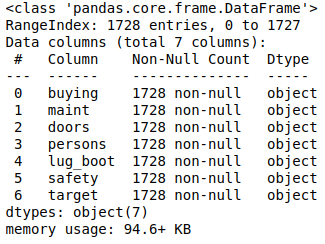
\includegraphics[scale = 0.45]{df_info.png}
\caption{Summary of the dataset}
\label{df_info}
\end{figure}

\begin{figure}[tbh]
\centering
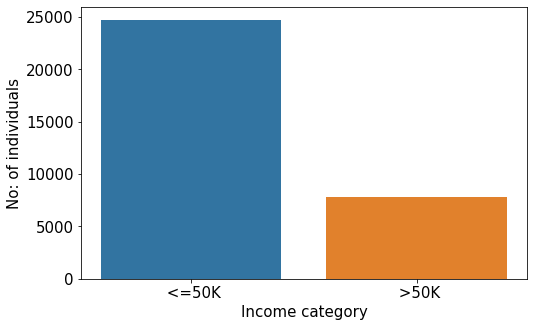
\includegraphics[scale = 0.47]{income_dist.png}
\caption{Target class imbalance}
\label{income_dist}
\end{figure}

\subsection{Feature by feature analysis}

For each feature, we perform the following analyses:

\begin{itemize}
    \item For continuous features, we first explore how the feature itself is distributed. For Gaussian Naive Bayes to be effective an important requirement is to have the variable distributed approximately normally.
    \item Then we make appropriate plots for continuous and categorical features to explore if we can derive any insights from a visual standpoint. Only features which provide insights are reported though all features were tested.
\end{itemize}

\subsection*{Continuous variables}

We make use of kernel density estimate (kde) plots for examining the distribution of continuous variables. KDE plots are essentially smoothed histograms. Since they are less cluttered versions of histogram plots, insights are more obvious. 

For applying naive bayes, it is essential to ensure that none of the continuous features are correlated. The correlation matrix is shown in Figure \ref{cont_corr}. \textbf{Clearly, the correlation values are very small, thereby validating the naive bayes assumption of independence of features.}

\begin{figure}[tbh]
\centering
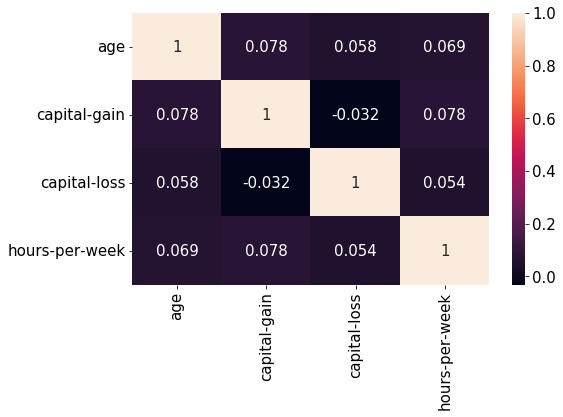
\includegraphics[scale = 0.43]{cont_corr.png}
\caption{Correlation for continuous features}
\label{cont_corr}
\end{figure}

We explore the continuous variables one by one below:

\subsection*{Age}

We obtain the plot as given in Figure \ref{age_kde}. Although the plot does resemble a Gaussian, it is skewed. In an attempt to make it more like a Gaussian, we can apply the box-cox transformation. It transforms a datapoint y as follows:

$$
    y(\lambda)= 
\begin{cases}
    \frac{y^{\lambda} - 1}{\lambda},& \text{if } \lambda \neq 0\\
    \log y,              & \text{if } \lambda = 0
\end{cases}
$$ $\lambda$ is treated as a hyper-parameter and the most suitable value is chosen. After performing the box-cox transformation, the age variable distribution gets transformed and the transformed feature is illustrated in Figure \ref{age_boxcox_kde}. Clearly, the distribution more closely resembles a Gaussian now. We will use this transformed quantity while applying Gaussian Naive Bayes.

\begin{figure}[tbh]
\centering
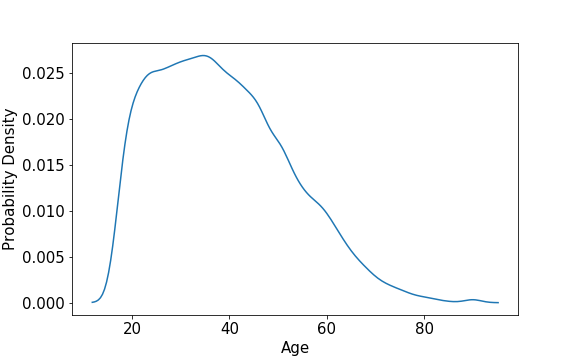
\includegraphics[scale = 0.43]{age_kde.png}
\caption{Density plot for Age}
\label{age_kde}
\end{figure}

\begin{figure}[tbh]
\centering
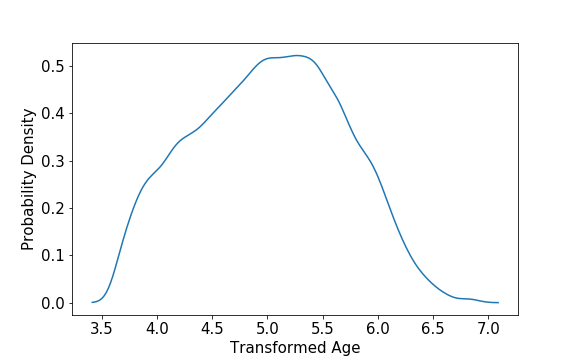
\includegraphics[scale = 0.43]{age_boxcox_kde.png}
\caption{Density plot for transformed age variable}
\label{age_boxcox_kde}
\end{figure}

On plotting the distribution of age according to income category, we obtain the plot in Figure \ref{incomevsage}. We observe that:

\begin{itemize}
    \item The \textbf{peak for income group $\leq$ 50K occurs close to the age 20.} This is intuitive as we expect people in their 20s to make less income as they are probably just starting out on jobs/ businesses.
    \item \textbf{The peak for income $>$ 50K occurs close to the age 40.} This is also intuitive as we expect most people to be at their peak earning capacity around this age. As they grow older, they move closer to retirement, possibly adversely affecting their income.
    \item We notice that there is a \textbf{greater proportion of people with income $\leq$ 50K as compared to $>$ 50K for any given age,} which is what we would expect from any society.
\end{itemize}

\begin{figure}[tbh]
\centering
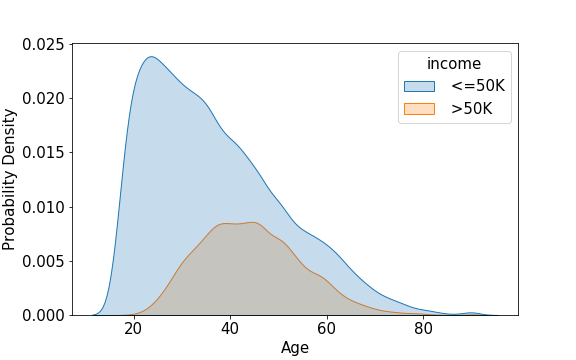
\includegraphics[scale = 0.43]{incomevsage.png}
\caption{Age distribution for different income categories}
\label{incomevsage}
\end{figure}


\subsection*{fnlwgt}

No description of this variable was given in the problem statement. After scouring the internet to find what this variable actually represents, the following description was found in the official dataset description:

"People with similar demographic characteristics should have similar weights.  There is one important caveat to remember about this statement.  That is that since the CPS sample is actually a collection of 51 state samples, each with its own probability of selection, the statement only applies within state."

However, we clearly have no information regarding which state an individual is from. \textbf{Hence, for our purposes, we can safely discard this variable} as this variable does not add any value, as long as we don't have any information regarding state. For the sake of completeness, the distribution of this variable is given in Figure \ref{fnlwgt_kde}.

\begin{figure}[tbh]
\centering
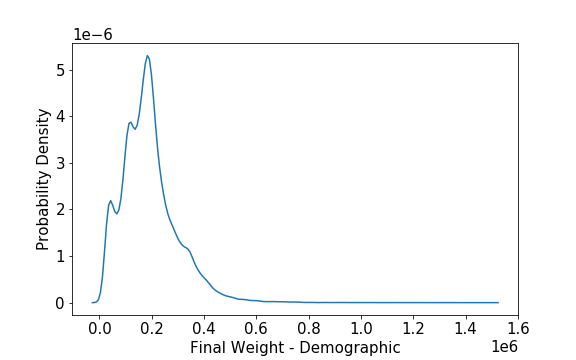
\includegraphics[scale = 0.43]{fnlwgt_kde.png}
\caption{Distribution of the variable fnlwgt}
\label{fnlwgt_kde}
\end{figure}

\subsection*{Years of education}

We obtain the distribution plot as given in Figure \ref{yoe_kde}. We see that the distribution doesn't resemble a Gaussian at all. We also note that whatever information is captured by years of education is also captured by the 'education' column, which is categorical and hence is easier to handle with naive bayes. So we drop this column and do not use it for Naive Bayes model.

On plotting the distribution of years of education according to income category, we obtain the plot in Figure \ref{incomevyoe}. We observe that in general, \textbf{people who earn more tend to have invested a longer duration in education.}

\begin{figure}[tbh]
\centering
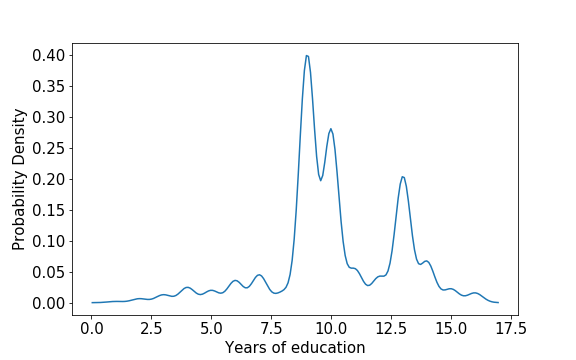
\includegraphics[scale = 0.43]{yoe_kde.png}
\caption{Distribution of the number of years of education}
\label{yoe_kde}
\end{figure}

\begin{figure}[tbh]
\centering
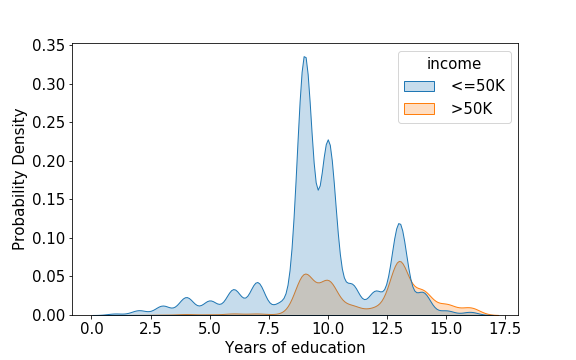
\includegraphics[scale = 0.43]{incomevyoe.png}
\caption{Number of years of education for different income categories}
\label{incomevyoe}
\end{figure}

\subsection*{Capital gain}

We obtain the distribution plot as given in Figure \ref{capgain_kde}. Although the right tail is longer than left tail, since the values are almost zero along the right tail, we consider this to be a Gaussian and hence do not apply any transform.

On plotting the distribution of capital gain according to income category, we obtain the plot in Figure \ref{capgainvsincome}. Capital gain plots don't seem to reveal any information regarding the dataset. This could be because more than 50\% of the points have the capital gain value as 0 as a majority of the population do not involve in capital asset transactions. So we try plotting only the non-zero values to see if we can infer anything. We obtain the plot given in Figure \ref{nonzero_capgainvsincome}. Clearly, we observe that a \textbf{higher capital gain has a higher probability density for people in the high income bracket,} which makes sense intuitively. 


\begin{figure}[tbh]
\centering
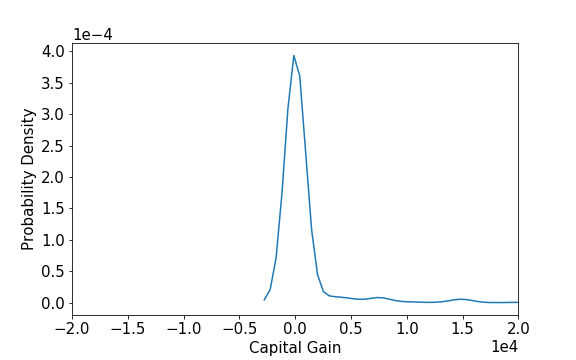
\includegraphics[scale = 0.43]{capgain_kde.png}
\caption{Distribution of the capital gain}
\label{capgain_kde}
\end{figure}

\begin{figure}[tbh]
\centering
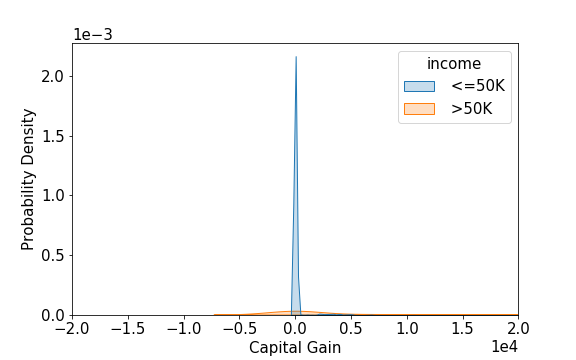
\includegraphics[scale = 0.43]{capgainvsincome.png}
\caption{Capital gain for different income categories}
\label{capgainvsincome}
\end{figure}

\begin{figure}[tbh]
\centering
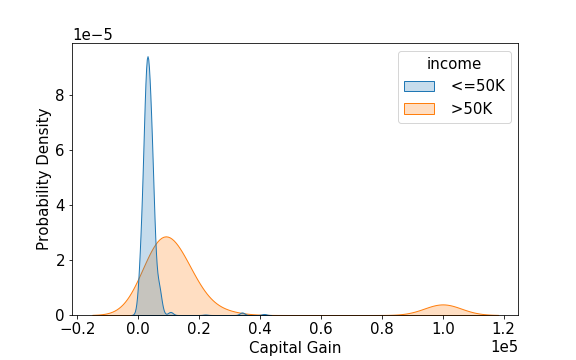
\includegraphics[scale = 0.43]{nonzero_capgainvsincome.png}
\caption{Capital gain considering only non-zero values}
\label{nonzero_capgainvsincome}
\end{figure}

\subsection*{Capital loss}

We obtain the distribution plot as given in Figure \ref{caploss_kde}. Again the right tail is longer than left tail, however since the values are almost zero along the right tail, we consider this to be a Gaussian and hence do not apply any transform.

 Since the situation is same as that of capital gain, so we try plotting only the non-zero values to see if we can infer anything. We obtain the plot given in Figure \ref{nonzero_caplossvsincome}. Counter-intuitively, it seems like people with higher income have higher capital losses on average!  However, this could be because the more you get involved in capital asset transactions, the more are your chances for gain/loss. Individuals could still be in the high income category if the gains offset losses.


\begin{figure}[tbh]
\centering
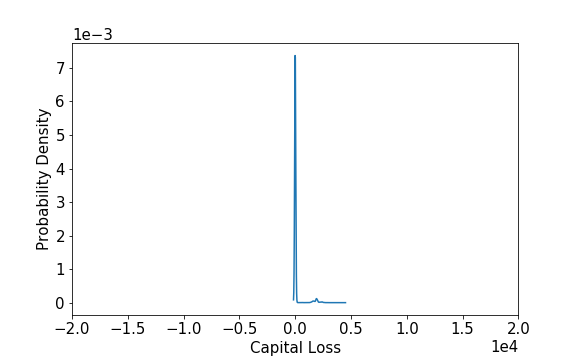
\includegraphics[scale = 0.43]{caploss_kde.png}
\caption{Distribution of the capital loss}
\label{caploss_kde}
\end{figure}


\begin{figure}[tbh]
\centering
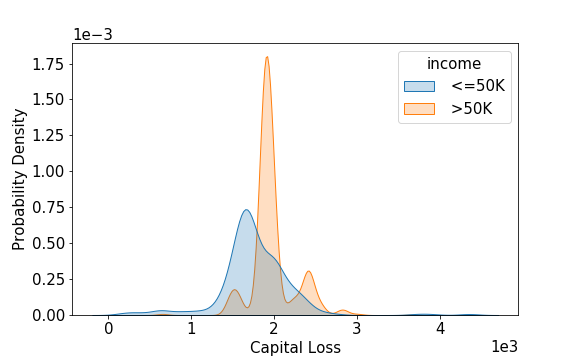
\includegraphics[scale = 0.43]{nonzero_caplossvsincome.png}
\caption{Capital loss considering only non-zero values}
\label{nonzero_caplossvsincome}
\end{figure}

\subsection*{Hours per week}

We obtain the distribution plot as given in Figure \ref{hpw_kde}. The distribution is sufficiently close to Gaussian, so we do not use any transforms.

On plotting the distribution of working hours per week according to income category, we obtain the plot in Figure \ref{incomevshpw}. We make the following observations:

\begin{itemize}
    \item Contrary to what one would expect, it appears that working more hours does not necessarily mean your income will be higher.
    \item However, it can be seen that a higher proportion of high income population works for more than 40 hours as compared to the lower income population.
\end{itemize}

\begin{figure}[tbh]
\centering
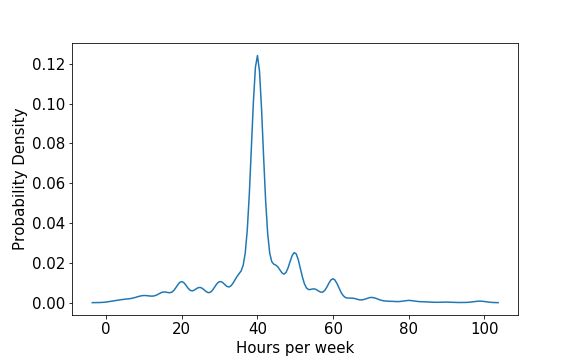
\includegraphics[scale = 0.43]{hpw_kde.png}
\caption{Distribution of the working hours per week}
\label{hpw_kde}
\end{figure}

\begin{figure}[tbh]
\centering
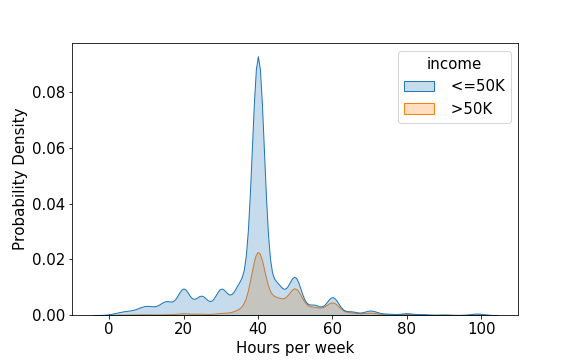
\includegraphics[scale = 0.43]{incomevshpw.png}
\caption{Working hours per week for different income categories}
\label{incomevshpw}
\end{figure}


\subsection*{Categorical variables}

For the case of categorical variables, we make use of count plots instead of kde plots for visualization. We plot the count of each category of a categorical variable according to the two income categories.

\subsection*{Working class}

We obtain the count plot as shown in Figure \ref{workclass_count}. We make the following observations:

\begin{itemize}
    \item Self-employed(inc) is the only category with more individuals belonging to high income category as compared to low income category. This shows that  you are more \textbf{likely to earn better if you manage to start a successful business for yourself.}
    \item Private sector has a high proportion of people from both high-income and low-income categories. This evidences the infamous \textbf{income disparity in the private sector.}
    \item There are some individuals for which the working class is denoted by ?'. These represent individuals for who we do not know the working class.
\end{itemize}

On examination, it is found that only 5.6\% of the total number of entries have the working class missing. Since the number is marginal, we drop these rows.

\begin{figure}[tbh]
\centering
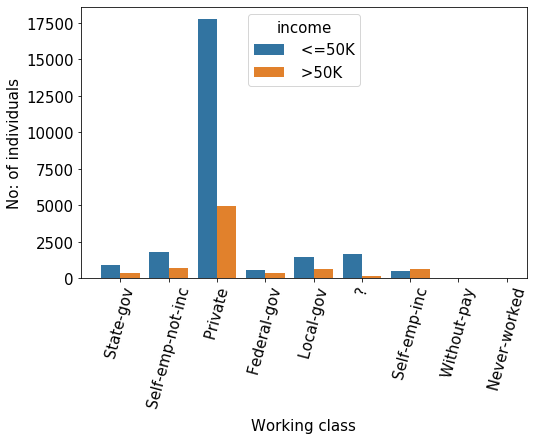
\includegraphics[scale = 0.43]{workclass_count.png}
\caption{Distribution of working class }
\label{workclass_count}
\end{figure}

\subsection*{Education}

We obtain the count plot as shown in Figure \ref{education_count}. We make the following observations:

\begin{itemize}
    \item Although we cannot make a blanket statement that education directly ensures high income, we see that the \textbf{only categories with proportion of high income group more than proportion of low income group are Masters and Doctorate groups.} 
    \item The proportion of high income individuals is very low for people who did not attend university, again implying that \textbf{education has a significant role in determining income.}
\end{itemize}


\begin{figure}[tbh]
\centering
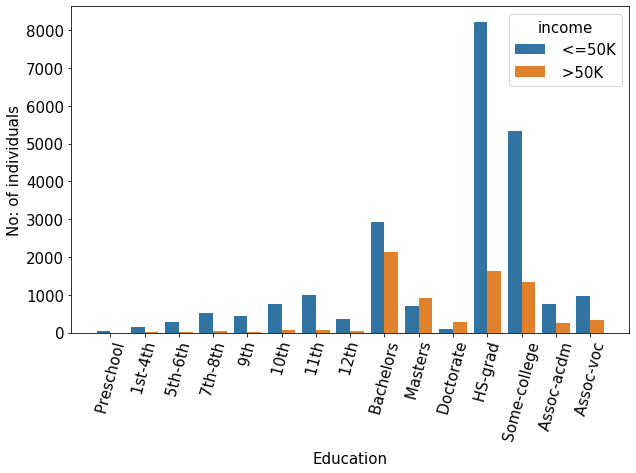
\includegraphics[scale = 0.39]{education_count.png}
\caption{Distribution of education levels }
\label{education_count}
\end{figure}

\subsection*{Marital status}

We obtain the count plot as shown in Figure \ref{marital_count}. We observe that Married-civ-spouse is the only category which has comparable number of people belonging to both categories of income. For other categories, the fraction of people belonging to high income category is marginal. This might be because married individuals may be more concerned about their financial security.


\begin{figure}[tbh]
\centering
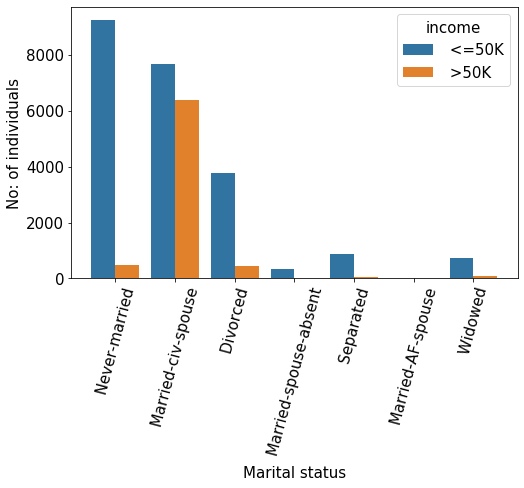
\includegraphics[scale = 0.43]{marital_count.png}
\caption{Distribution of marital status }
\label{marital_count}
\end{figure}

\subsection*{Occupation}

We obtain the count plot as shown in Figure \ref{occupation_count}. We observe that \textbf{managerial executives and speciality professionals are likely to earn more.} This also makes sense intuitively as these are often considered as the "high-paying" professions.


\begin{figure}[tbh]
\centering
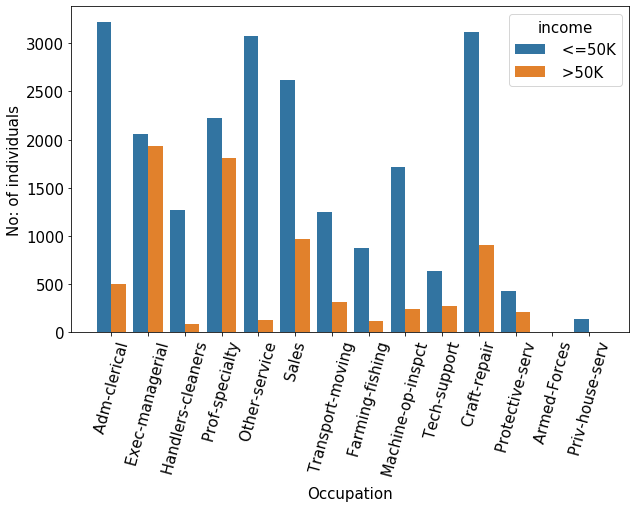
\includegraphics[scale = 0.39]{occupation_count.png}
\caption{Distribution of occupation }
\label{occupation_count}
\end{figure}

\subsection*{Gender}

We obtain the count plot as shown in Figure \ref{sex_count}. We observe that \textbf{on an average, males have more chance to earn more than females,} and that about a third of males earn more than 50k income.


\begin{figure}[tbh]
\centering
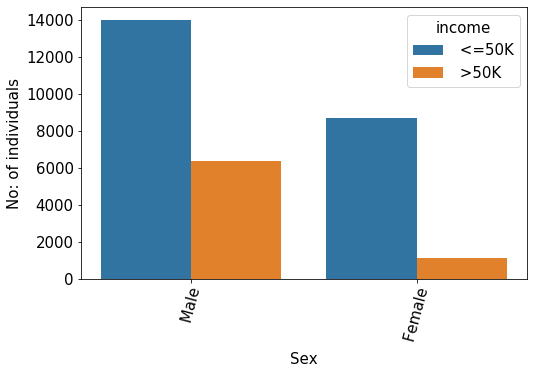
\includegraphics[scale = 0.43]{sex_count.png}
\caption{Distribution of gender/sex }
\label{sex_count}
\end{figure}

\section{Model: Naive Bayes Classifier}

In this section, we will give a brief overview of the mathematical formalism behind the naive bayes classifier. 

Naive Bayes classifiers are a family of simple "probabilistic classifiers" based on applying Bayes' theorem with \textbf{strong (naive) independence assumptions between the features.}Naive Bayes classifiers are \textbf{highly scalable}, requiring a number of parameters linear in the number of variables/features in a learning problem. Maximum-likelihood training, which is the most generally used strategy, can be done by \textbf{evaluating a closed-form expression} which takes linear time, rather than by expensive iterative approximation, such as gradient descent, as used for many other types of classifiers. Despite the seemingly strong assumptions, naive bayes classifiers have been shown to work well in a lot of real-life scenarios.

\subsection{Probabilistic Model}

In any classification problem, our goal is to find the class $C_k$ in which a given  datapoint \textbf{x}, which will be an n-dimensional vector, where n is the number of features, belongs. Then, more formally, our goal is to find $P(C_k|\mathbf{x})$ for each class $C_k$.

Using Bayes' theorem,

$$ P(C_k|\mathbf{x}) = \frac{P(C_k, \mathbf{x})}{P(\mathbf{x})} $$ For a given datapoint, the denominator is fixed, implying that the class to which the point should be assigned is influenced solely by the numerator which essentially contains the joint probability function $P(C_k, \mathbf{x})$. Now,

$$ P(C_k, \mathbf{x}) = P(C_k, x_1, x_2, ..., x_n)$$ where $x_1, x_2..., x_n$ are the n features. \textbf{This is where we make use of the strong naive bayes assumption of mutual independence of features, conditional on the class $C_k$} Using this assumption,

$$P(C_k, x_1, x_2, ..., x_n) = P(C_k)P(x_1|C_k)P(x_2|C_k)...P(x_n|C_k)$$ Therefore, we can write:

$$ P(C_k|\mathbf{x}) \propto  P(C_k) \Pi_{i=1}^{n}P(x_i|C_k)$$ $P(C_k)$ is termed the \textbf{prior probability} for class $C_k$, since this can be interpreted as the probability of observing class $C_k$ before any observations were made. If we know the distribution of the classes before measurements through some \textbf{domain knowledge, this can be used for assigning the prior probabilities.} If not, we can always choose a uniform prior which would mean assigning equal probabilities to all classes.

By making the simplifying assumption of independence of features, we are required to compute only the distributions $P(x_i|C_k)$ for $i \in \{1, 2, ...,n\}$, instead of the joint distribution. How does this make the computations easier?

To see this, let us assume all distributions are normal. If we do not assume conditional independence, we will be required to compute $P(x_1, x_2,..., x_n|C_k)$ which essentially is a joint Gaussian having $n$ variables. Clearly, the covariance matrix of such a Gaussian will $n^2$ entries and hence the estimation of parameters will be $O(n^2)$. However, if we assume independence, this can be broken down into n separate Gaussians with just 1 variable each. Clearly, such a model would only require $O(n)$ parameter estimations, giving us a \textbf{quadratic speedup}. This can immensely help in computations, especially while dealing with reasonably large datasets.

Notice that this simplifying assumption reduces the complexity of the model. This makes naive bayes a \textbf{high bias, low variance classifier.} 

\textbf{Typically, for continuous features we assume the distribution to be Gaussian and for categorical variables, we assume the distribution to be bernoulli/categorical distribution.} After choosing a distribution, we estimate the parameters using Maximum Likelihood Estimation.


\subsection{MAP decision rule}

After obtaining the probabilities $P(C_k|\mathbf{x})$, we must make a prediction to assign a class. The most commonly used prediction strategy is to \textbf{pick the class with the highest value} of $P(C_k|\mathbf{x})$. This is termed as the  maximum a posteriori or MAP decision rule.

\subsection{Gaussian Naive Bayes}

Gaussian Naive Bayes is a typically used model for continuous variables. We essentially assume the Gaussian distribution:

$$ f_x(x|C_k) = \frac{1}{\sqrt{2\pi}{\sigma}_k}e^{\frac{-(x-{\mu}_k)^2}{2{\sigma}^2_k}} $$ for the probability density function for class $C_k$. 

We estimate ${\mu}_k$, ${\sigma}_k$ and the prior ${\pi}_k$($P(C_k)$)for each class $C_k$ as follows:

$$ \hat{\mu}_k = \frac{\sum_{i \forall n_k}x_i}{n_k} $$
$$ \hat{\sigma}_k^2 = \frac{\sum_{i \forall n_k}(x_i - \hat{\mu}_k)^2}{n_k - 1} $$
$$ \hat{\pi}_k = \frac{n_k}{n} $$ where $n_k$ is the number of observations of the $\textrm{k}^\textrm{th}$ class and $n$ is the total number of observations. 

If we assume shared variances across the different classes, we will obtain \textbf{linear decision boundaries.}

\subsection{Categorical Naive Bayes}

When the input feature is categorically distributed, we use categorical naive bayes. In categorical naive bayes, we assume the probability distribution for each feature to be a categorical variable. Suppose a feature$x_j$ can take values in categories ${1, 2, ..., T}$. Then mathematically, the probability for feature $x_j$ to take value as category $t$, given a class $C_k$ is estimated as:

$$ P(x_j=t|C_k) =  \frac{N_{kt}}{N_k}$$ where $N_{kt}$ is the number of samples in class $C_k$ which have category of $x_j$ as $t$ and $N_k$ is the total number of samples in class $C_k$. We then calculate the probability of observing the sample $X_i$ given a class $C_k$ by multiplying out the above calculated probabilities for each feature.

However, this approach has one drawback: if we encounter a category which we have never seen before, the entire product vanishes because the probability for this particular category goes to zero. To prevent this, a smoothing parameter $\alpha$, which is typically a small value greater than zero, is added to both the numerator and denominator:

$$ P(x_j=t|C_k) =  \frac{N_{kt} + \alpha}{N_k + \alpha}$$

$$  $$

\section{Modelling }

In this section, we discuss the application of the naive bayes classifier to our problem. 

We create and evaluate two separate models:

\begin{enumerate}
    \item In Model 1, we \textbf{set the prior uniformly for both classes,} i.e., we assign 0.5 each for the prior values.
    \item In Model 2, we \textbf{set the prior according to the class distribution,} i.e we set 0.751 for the low-income category and 0.249 for the high-income category.
\end{enumerate}

Each model is generated using a \textbf{"mixed" naive bayes approach.} This is because we have both numerical and categorical variables. So we fit a Gaussian naive bayes classifier on the continuous features, a categorical naive bayes classifier on the categorical features, get the output probabilities and multiply them out to get the total probabilities from the model.

We evaluate the models based on multiple metrics. A short description of the used metrics is given below:

\begin{itemize}
    \item \textbf{Accuracy:}
    Accuracy is simply the \textbf{ratio of number of correct predictions to total number of predictions.} Although this seems like a very good metric intuitively, accuracy fails on classification problems with a skewed class distribution because of the intuitions developed by practitioners on datasets with an equal class distribution.
    \item \textbf{Precision:}
    Precision is the \textbf{ratio of true positives to the total positive predictions.} Precision is typically used when the cost of false positive is high. For instance, email spam detection.
    \item \textbf{Recall:}
    Precision is the \textbf{ratio of true positives to the total positive ground truths.} Recall is typically used when the cost of false negative is high. For instance, in fraud detection or sick patient detection.
    \item \textbf{F1-score:}
    F1-score is simply a \textbf{harmonic average of precision and recall.} F1 Score is typically used if we need to seek a balance between Precision and Recall and there is an uneven class distribution.
    
    
\end{itemize}

\subsection{Model 1}

The confusion matrix for model 1 is shown in Figure \ref{cmwithoutprior}. The values for the evaluation metrics are given in Table \ref{noprior_metric_table}.

\begin{figure}[tbh]
\centering
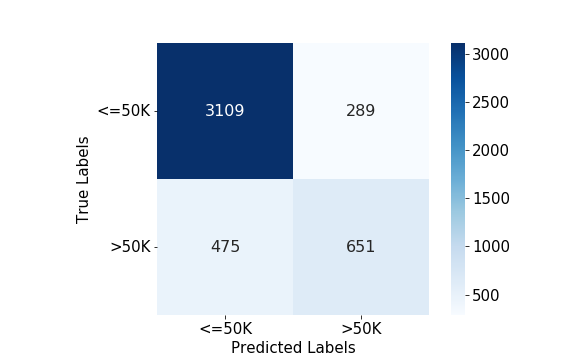
\includegraphics[scale = 0.42]{cmwithoutprior.png}
\caption{Confusion matrix for model 1 (uniform prior)}
\label{cmwithoutprior}
\end{figure}

\begin{table}
\begin{center}

\caption{Metrics for model 1 (uniform prior)}

\begin{tabular}{| c| c| }
 \hline
 Metric & Score \\
 \hline
 \hline
 Accuracy & 0.831 \\ 
 \hline
 Precision & 0.692 \\   
 \hline
 Recall & 0.578 \\
 \hline
 F1 Score & 0.630 \\
 \hline

\end{tabular}

\label{noprior_metric_table}
\end{center}

\end{table}

\subsection{Model 2}

The confusion matrix for model 2, using prior based on class distribution, is shown in Figure \ref{cmwithprior}. The values for the evaluation metrics are given in Table \ref{prior_metric_table}.

\begin{figure}[tbh]
\centering
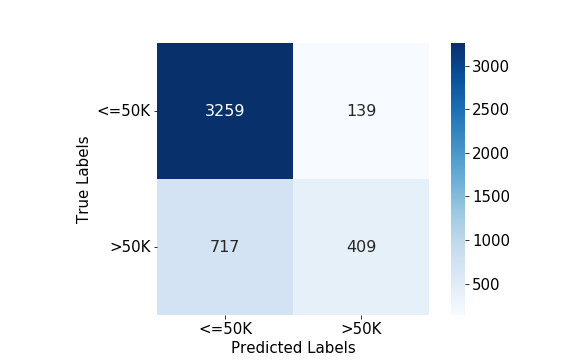
\includegraphics[scale = 0.42]{cmwithprior.png}
\caption{Confusion matrix for model 2 (non-uniform prior)}
\label{cmwithprior}
\end{figure}

\begin{table}
\begin{center}

\caption{Metrics for model 2 (non-uniform prior)}

\begin{tabular}{| c| c| }
 \hline
 Metric & Score \\
 \hline
 \hline
 Accuracy & 0.811 \\ 
 \hline
 Precision & 0.746 \\   
 \hline
 Recall &  0.363 \\
 \hline
 F1 Score & 0.489 \\
 \hline

\end{tabular}

\label{prior_metric_table}
\end{center}

\end{table}

We observe that \textbf{Model 2 has better precision whereas Model 1 performs better in all other metrics.} Although we might consider Model 2 in settings where precision is of utmost importance, in this case since Model 1 does better in all other aspects, we choose \textbf{Model 1 to be the better model.}

ROC curve is another common tool used with binary classifiers. A Receiver Operating Characteristic curve, or ROC curve, is a graphical plot that illustrates the diagnostic ability of a binary classifier system as its discrimination threshold is varied. The ROC curve is created by plotting the true positive rate (TPR) against the false positive rate (FPR) at various threshold settings. The ROC curve for Model 1 is given in Figure \ref{Roccurve}.

\begin{figure}[tbh]
\centering
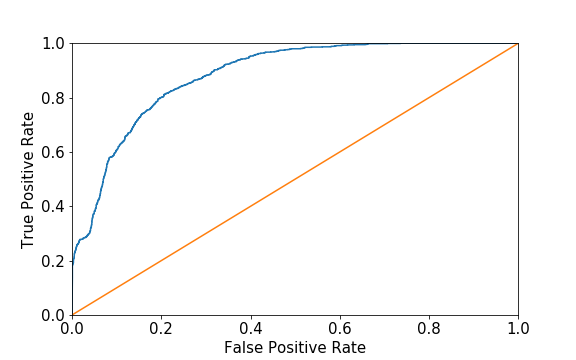
\includegraphics[scale = 0.43]{Roccurve.png}
\caption{ROC curve for Model 1}
\label{Roccurve}
\end{figure}

The dotted line represents the ROC curve of a purely random classifier; a good classifier stays as far away from that line as possible (toward the top-left corner). One way to compare classifiers is to measure the area under the curve (AUC). A perfect classifier will have a ROC AUC equal to 1, whereas a purely random classifier will have a ROC AUC equal to 0.5. \textbf{The area under the ROC curve of our naive bayes classifier is 0.882.}

To get a sense of how much continuous variables and categorical variables contribute to the prediction quality, we take the Gaussian naive bayes and categorical naive bayes (with uniform prior) separately and make predictions. For Gaussian naive bayes, we obtain the confusion matrix shown in Figure \ref{cm_gaussian} and metrics shown in Table \ref{gauss_metric_table}. For categorical naive bayes, we obtain the confusion matrix shown in Figure \ref{cm_cat} and metrics shown in Table \ref{cat_metric_table}.

From the confusion matrix as well as the metrics, it is clear that the Gaussian naive bayes contributes mostly to the precision metric whereas the categorical naive bayes dominates all other metrics. If we were to choose between the two, \textbf{categorical naive bayes is more relevant as it leads to a more balanced model. Hence, we can conclude that the categorical variables contribute more to the income category prediction.}

\begin{figure}[tbh]
\centering
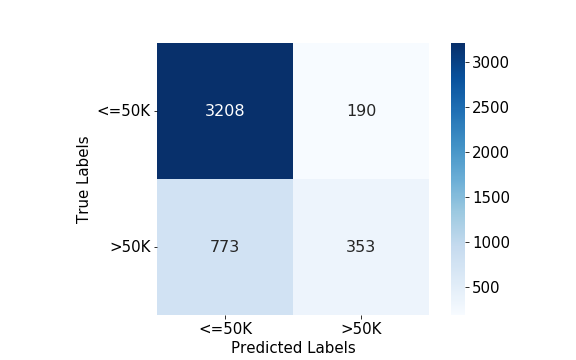
\includegraphics[scale = 0.42]{cm_gauss.png}
\caption{Confusion matrix for Gaussian naive bayes}
\label{cm_gaussian}
\end{figure}

\begin{table}
\begin{center}

\caption{Metrics for Gaussian naive bayes}

\begin{tabular}{| c| c| }
 \hline
 Metric & Score \\
 \hline
 \hline
 Accuracy & 0.787 \\ 
 \hline
 Precision & 0.650 \\   
 \hline
 Recall &  0.313 \\
 \hline
 F1 Score & 0.423 \\
 \hline

\end{tabular}

\label{gauss_metric_table}
\end{center}

\end{table}

\begin{figure}[tbh]
\centering
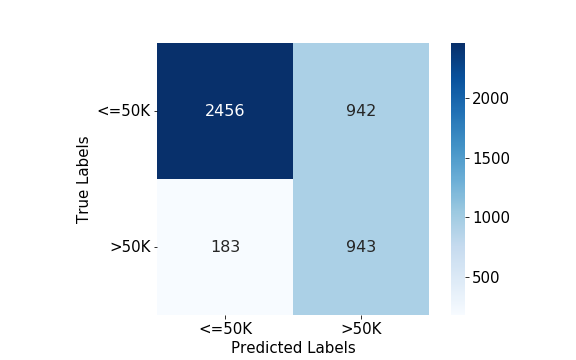
\includegraphics[scale = 0.42]{cm_cat.png}
\caption{Confusion matrix for categorical naive bayes}
\label{cm_cat}
\end{figure}

\begin{table}
\begin{center}

\caption{Metrics for categorical naive bayes}

\begin{tabular}{| c| c| }
 \hline
 Metric & Score \\
 \hline
 \hline
 Accuracy & 0.751 \\ 
 \hline
 Precision & 0.500 \\   
 \hline
 Recall &  0.837 \\
 \hline
 F1 Score & 0.626 \\
 \hline

\end{tabular}

\label{cat_metric_table}
\end{center}

\end{table}

\section{Conclusions}

From our extensive analysis of the given dataset using naive bayes calssifier, we arrive at the following conclusions:

\begin{itemize}
    \item Naive bayes classifier, despite having rather strong assumptions, performs reasonably well as long as the features are more or less independent and the continuous variables are approximately Gaussian.
    \item Changing the prior can significantly affect the performance of the naive bayes model as evidenced by the improvement in performance using a uniform prior instead of class weighted prior.
    \item Categorical features provide more insights regarding the value of target variable as compared to continuous features as is evident from the fact that the categorical naive bayes classifier outperforms the Gaussian naive bayes classifier.
    \item The income bracket of an individual can be predicted to a reasonable extent using factors like education, age, profession and gender.
    \item While it is acceptable that education and working hours influence the income, it must be critically examined if certain groups based on gender and race face barriers while aspiring to be in the high income category to ensure wellness and propserity of the society as a whole.
\end{itemize}



\section{Avenues for further research}

Naive bayes classifier, despite working reasonably well, has very strong assumptions which might not be warranted in many cases. Using other models like SVM which do not require such strong assumptions might lead to better results. Further, rather than using Gaussian naive bayes, if we can more accurately model the distribution of continuous variables, we might be able to achieve better performance.



\nocite{*} % Print all references regardless of whether they were cited in the poster or not
\bibliographystyle{ieeetr}
\bibliography{sample} % Use the example bibliography file sample.bib


\end{document}

